\textnormal{
Describing of a User Interface (UI) to the system along with the related information that will be shown on each screen (How users will query the tables and view the query results). The emphasis should be placed on the process required for a user in order to meet a particular information need, in a user-friendly manner.
The deliverables for this stage include the following items (Please refer to the original Project Description for more details):
\begin{itemize} 
\item{}
	The SQL statements used to query the data. 
\item{}
	The error messages that will pop-up when users access and/or updates are denied.
\item{}
	The error messages corresponding to the integrity constraints violations.
\item{}
	The error messages corresponding to the data range constraints violations.
\item{}
	The header of the views created in order to facilitate data accesses, according to users'  needs. 
\item{}
	Each view created must be justified. Any triggers built upon those views should be explained and justified as well. At least one view should be created and justified for the project.
\end{itemize}
Please insert your deliverables for Stage4 as follows:
\begin{itemize} 
\item{The the first SQL statement used to query the data: }
	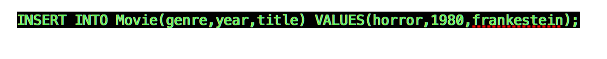
\includegraphics[scale=0.3]{insert1.png}
\item{The tables taking part in the query statement (table names and headers): }
	Please insert the tables taking part in the query statement, as follows.
	 \begin{itemize} 
	 \item{The name of the first table taking part in the query: }
	 Movie
	  \item{The header of the table  (all attributes): }
	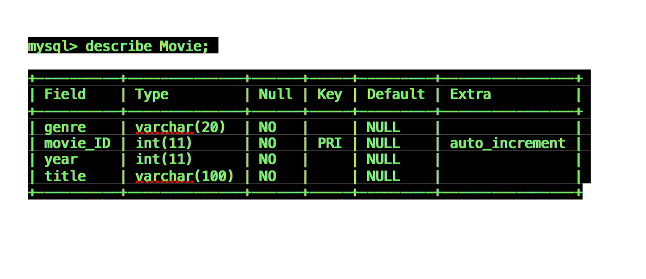
\includegraphics[scale=0.3]{describemovie.png}
	  \item{The attributes of the table taking part in the query: }
	  genre,year,title
	 \end{itemize}
\item{}
	The error messages popping-up when users access and/or updates are denied (along with explanations and examples):
	\begin{itemize} 
	\item{The error message: }
	ERROR 1142(42000): INSERT command denied to user ?moviegoer?@?localhost? for table ?Movie?
	\item{The error message explanation (upon which violation does it take place): }
	When a moviegoer tries to make changes to the movie information, this will be denied because the moviegoer does not have access to movie information
	\item{The error message example according to user(s) scenario(s): }
	When a moviegoer user tries to make add a movie to the movie table because he wants to add one of his favorite movies that arent showing in any of theaters , he/she tries to add it and the error message will pop-up.
	 \end{itemize}
\item{The the first SQL statement used to query the data: }
	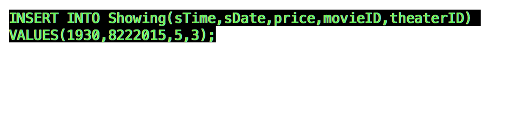
\includegraphics[scale=0.3]{insert2.png}
\item{The tables taking part in the query statement (table names and headers): }
	Please insert the tables taking part in the query statement, as follows.
	 \begin{itemize} 
	 \item{The name of the first table taking part in the query: }
	 Showing
	  \item{The header of the table  (all attributes): }
	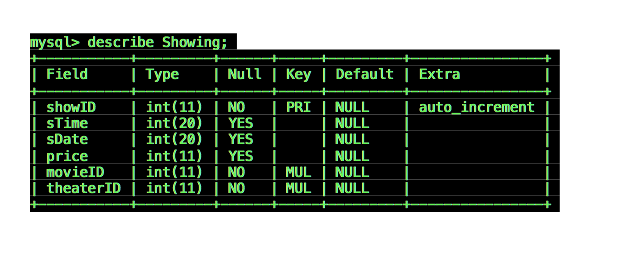
\includegraphics[scale=0.3]{desshowing.png}
	  \item{The attributes of the table taking part in the query: }
	  showID,sTime,sDate,price,movieID,theaterID
	 \end{itemize}
\item{}
	The error messages popping-up when users access and/or updates are denied (along with explanations and examples):
	\begin{itemize} 
	\item{The error message: }
	 ERROR 1142(42000): INSERT command denied to user ?moviegoer?@?localhost? for table ?Showing?
	\item{The error message explanation (upon which violation does it take place): }
	When a moviegoer tries to make changes to the showing information, the require will be denied because the moviegoer do not have access to showing information
	\item{The error message example according to user(s) scenario(s): }
	When a moviegoer user tries to make changes to showing information to mess with one of the theaters, the error message will pop-up.
	 \end{itemize}
\item{The the first SQL statement used to query the data: }
	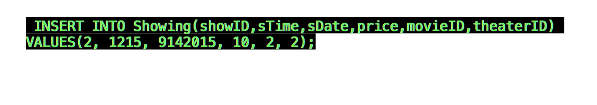
\includegraphics[scale=0.3]{IC.png}
\item{The tables taking part in the query statement (table names and headers): }
	Please insert the tables taking part in the query statement, as follows.
	 \begin{itemize} 
	 \item{The name of the first table taking part in the query: }
	Showing
	\item{The header of the table  (all attributes): }
	Showing(showID,sTime,sDate,price,movieID,theaterID)
	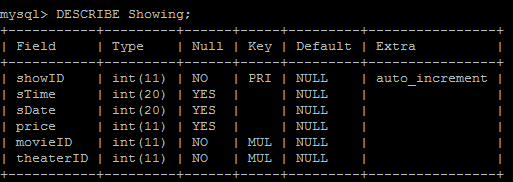
\includegraphics[scale=0.3]{m.png}
	  \item{The attributes of the table taking part in the query: }
	 showID,sTime,sDate,price,movieID,theaterID
	 \end{itemize}
	 Please repeat that pattern for all tables taking part in that query.
\item{}
	The error messages corresponding to the integrity constraints violations (along with explanations and examples).
	\begin{itemize} 
	\item{The error message: }
	"Cannot duplicate an ID; must be unique."
	\item{The error message explanation (upon which violation does it take place): }
	This error is for when a user tries to make a new movie showing with a showing ID that is already used for another showing.  This violates the primary key intergrity constraint.
	\item{The error message example according to user(s) scenario(s): }
	An employee tries to create a showing with an already existing ID.  The error message catches this and explains that each showing must have its own ID.
	 \end{itemize}
\item{The the first SQL statement used to query the data: }
	
\includegraphics[scale=0.3]{sql.png}
\item{The tables taking part in the query statement (table names and headers): }
	Please insert the tables taking part in the query statement, as follows.
	 \begin{itemize} 
	 \item{The name of the first table taking part in the query: }
	 Rate
	 \item{The header of the table  (all attributes): }
	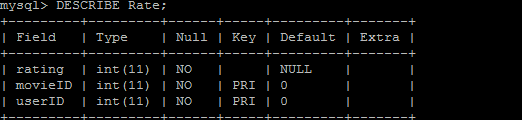
\includegraphics[scale=0.3]{mm.png}
	 \item{The attributes of the table taking part in the query: }
	  rating,movieID,userID
	 \end{itemize}
\item{}
	The error messages corresponding to the integrity constraints violations (along with explanations and examples).
	\begin{itemize} 
	\item{The error message: }
	Null was entered into a field that cannot be null
	\item{The error message explanation (upon which violation does it take place): }
	This error is for when a user tries to rate a movie without specifying a movie ID.  This violates the integrity constraint that each rating must be for exactly one movie.
	\item{The error message example according to user(s) scenario(s): }
	 A user enters a rating, but does not specify the movie that the rating is for.  Since the rating has to belong to a movie, that action is not allowed
	 \end{itemize}
\item{The the first SQL statement used to query the data: }
	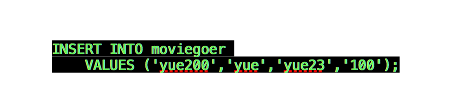
\includegraphics[scale=0.3]{insertData.png}
\item{The tables taking part in the query statement (table names and headers): }
	Please insert the tables taking part in the query statement, as follows.
	 \begin{itemize} 
	 \item{The name of the first table taking part in the query: }
	 Moviegoer
	  \item{The header of the table  (all attributes): }
	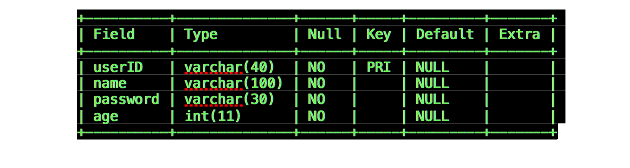
\includegraphics[scale=0.3]{moviegoerdescribe.png}
	  \item{The attributes of the table taking part in the query: }
	  userID, name, password, age
	 \end{itemize}
\item{}
	The error messages corresponding to the data range constraints violations (along with explanation).
	\begin{itemize} 
	\item{The error message: }
	invalid age
	\item{The error message explanation (upon which violation does it take place): }
	1 to 100 is accepted because a person who normally goes to movies can be between 1 and 100
	\item{The error message example according to user(s) scenario(s): }
	When a user types in their age when they are filling out their information we need, and they accidentally type 555 instead of 55 , the error message will pop up.
	 \end{itemize}
\item{The the first SQL statement used to query the data: }
	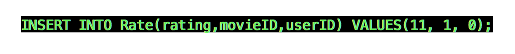
\includegraphics[scale=0.3]{ICC.png}
\item{The tables taking part in the query statement (table names and headers): }
	Please insert the tables taking part in the query statement, as follows.
	 \begin{itemize} 
	 \item{The name of the first table taking part in the query: }
	 Rate
	  \item{The header of the table  (all attributes): }
	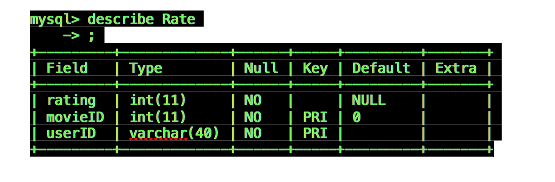
\includegraphics[scale=0.3]{rate.png}
	  \item{The attributes of the table taking part in the query: }
	  rating,movieID,userID
	  \end{itemize}
\item{}
	The error messages corresponding to the data range constraints violations (along with explanation).
	\begin{itemize} 
	\item{The error message: }
	invalid rating
	\item{The error message explanation (upon which violation does it take place): }
	rating is allowed from number 1 to 10 . if the moviegoer liked the movie then he/she would give it a 10 , otherwise if he/she did not like it at all they can give it a 1. rating between 1 and 10 no more or less, because it is usually one of the common scales out there, whereas if its 1 to 100 rating 
	\item{The error message example according to user(s) scenario(s): }
	if someone really liked a movie and wants to give them 100 rating , it will not be allowed because it would not be fair to the other movies, and it is not allowed because it is not the 1-10 common scale we are using for this theater management  
	 \end{itemize}
\item{The header of the views created in order to facilitate data accesses:}
Please insert the header of the views as follows:
\begin{itemize} 
	\item{The view created: }
	forMoviegoer
	\item{The view justification: }
	This view is built for moviegoer. When moviegoers log in, they have access to read all the movie information.
	\item{The tables taking part in the view and the specific attributes taking part in the view: }
	Please insert the tables names, headers, and the attributes as follows.
	\begin{itemize} 
		\item{The table name: }
		Movie
		\item{The table header (all attributes): }
		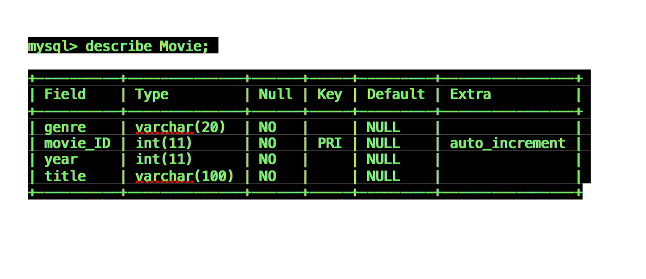
\includegraphics[scale=0.3]{describemovie.png}
		\item{The table attributes that take part in the view: }
		title, genre, year
	\end{itemize}
	\begin{itemize} 
		\item{The table name: }
		Showing
		\item{The table header (all attributes): }
		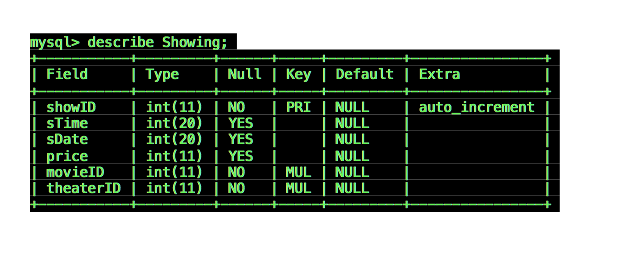
\includegraphics[scale=0.3]{desshowing.png}
		\item{The table attributes that take part in the view: }
		 sTime, sDate, price
	\end{itemize}
	\begin{itemize} 
		\item{The table name: }
		Director
		\item{The table header (all attributes): }
		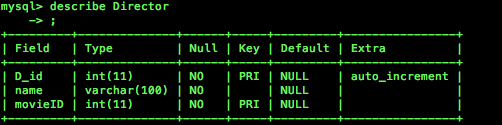
\includegraphics[scale=0.3]{director.png}
		\item{The table attributes that take part in the view: }
		directorname.
	\end{itemize}
	\begin{itemize} 
		\item{The table name: }
		Rate
		\item{The table header (all attributes): }
		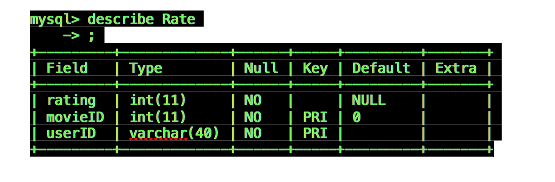
\includegraphics[scale=0.3]{rate.png}
		\item{The table attributes that take part in the view: }
		rating
	\end{itemize}
	Please repeat that pattern for every table that takes part in the view.
	\item{The SQL statement used for creating the view: }
	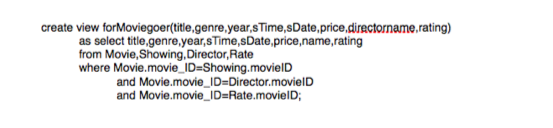
\includegraphics[scale=0.3]{VIEWMOVIEGOER.png}
	\item{The trigger built upon those views (if any): }
	Please insert the triggers as follows.
	\begin{itemize} 
		 \item{The trigger: }
		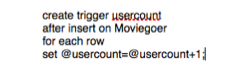
\includegraphics[scale=0.3]{trigger2.png}
		 \item{The trigger justification (explanation, correlating it to user scenario(s)): }
		a count that is added 1 after every insert on the moviegoer table to count how many moviegoers are in the system.the theater manager can see how many moviegoers are in his theater ?,he can just summon this trigger customer count 
 	\end{itemize}
\end{itemize}
Please, in case you have more than one view, repeat that pattern for each view.
\begin{itemize} 
	\item{The view created: }
	forTheatreManager
	\item{The view justification: }
	This view is built for theatre manager. When theatre manager log in, they have access to read all the movie information, showing information and the associated moviegoer information.
	\item{The tables taking part in the view and the specific attributes taking part in the view: }
	Please insert the tables names, headers, and the attributes as follows.
	\begin{itemize} 
		\item{The table name: }
		Movie
		\item{The table header (all attributes): }
		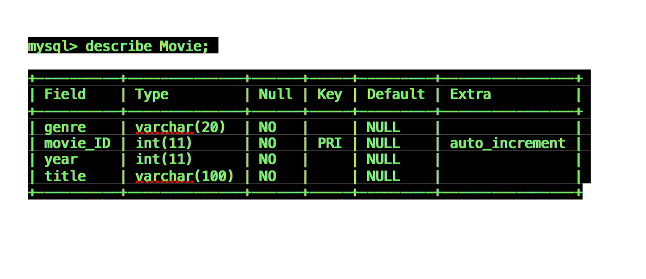
\includegraphics[scale=0.3]{describemovie.png}
		\item{The table attributes that take part in the view: }
		title, genre, year
	\end{itemize}
	\begin{itemize} 
		\item{The table name: }
		Showing
		\item{The table header (all attributes): }
		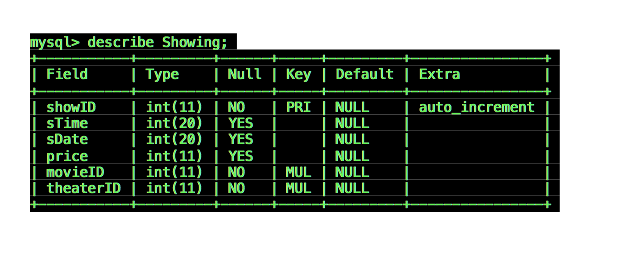
\includegraphics[scale=0.3]{desshowing.png}
		\item{The table attributes that take part in the view: }
		sTime, sDate, price
	\end{itemize}
	\begin{itemize} 
		\item{The table name: }
		Director
		\item{The table header (all attributes): }
		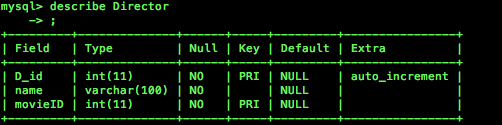
\includegraphics[scale=0.3]{director.png}
		\item{The table attributes that take part in the view: }
		directorname
	\end{itemize}
	\begin{itemize} 
		\item{The table name: }
		Moviegoer
		\item{The table header (all attributes): }
		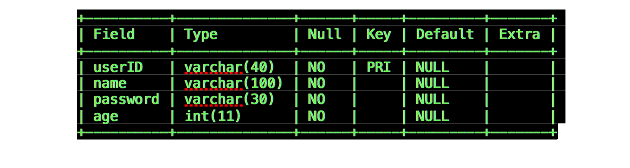
\includegraphics[scale=0.3]{moviegoerdescribe.png}
		\item{The table attributes that take part in the view: }
		username,age
	\end{itemize}
	\begin{itemize} 
		\item{The table name: }
		HasTicket
		\item{The table header (all attributes): }
		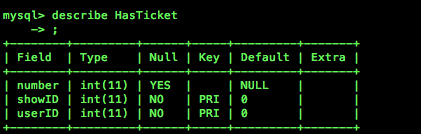
\includegraphics[scale=0.3]{hasticket.png}
		\item{The table attributes that take part in the view: }
		number.
	\end{itemize}
	Please repeat that pattern for every table that takes part in the view.
	\item{The SQL statement used for creating the view: }
	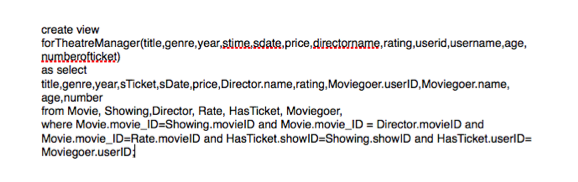
\includegraphics[scale=0.3]{VIEWTHEATER.png}
	\item{The trigger built upon those views (if any): }
	Please insert the triggers as follows.
	\begin{itemize} 
		 \item{The trigger: }
		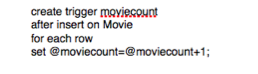
\includegraphics[scale=0.3]{trigger1.png}
		 \item{The trigger justification (explanation, correlating it to user scenario(s)): }
		 a count variable in which one is added every time a movie is added to the system so any of the managers can know how many movies are added to their movie theater system. a theater manager can check how many movies his theater has 
 	\end{itemize}
\end{itemize}
\end{itemize}
}
